% Copyright 2017-2019 Jean-Luc Vay, Remi Lehe
%
% This file is part of WarpX.
%
% License: BSD-3-Clause-LBNL


\usepackage{bm}
\usepackage{amsmath}
\usepackage{amssymb}
\usepackage{graphicx}
\usepackage{url}
\usepackage{hyperref}

\usepackage[displaymath]{lineno}\usepackage{bm}% bold math

\newcommand{\fe}{\mathbf{\tilde{E}}}
\newcommand{\fb}{\mathbf{\tilde{B}}}
\newcommand{\fj}{\mathbf{\tilde{J}}}
\newcommand{\ff}{\tilde{F}}
\newcommand{\fg}{\tilde{G}}
\newcommand{\fk}{\mathbf{k}}
\newcommand{\fkhat}{\mathbf{\hat{k}}}

% Definitions from Remi's paper on Galilean math
\newcommand{\Km}{\vec{K}_{\vec{m}}}
\newcommand{\km}{\vec{k}_{\vec{m}}}
\renewcommand{\vec}[1]{\boldsymbol{#1}}
\newcommand{\vgal}{\vec{v}_{gal}}
\newcommand{\nab}{\vec{\nabla'}}
\newcommand{\Dt}[1]{ \frac{\partial #1}{\partial t}}
\newcommand{\mc}[1]{\hat{\mathcal{#1}}}
\newcommand{\xj}{\vec{x}'_{\vec{j}}}
\newcommand{\Xll}{\vec{X}_{\vec{\ell}}}
\newcommand{\Integ}[1]{\int_{-\infty}^{\infty} \!\!\!\!\!\!
  \mathrm{d}#1}
\newcommand{\RInteg}[1]{\int_{0}^{\infty} \!\! \frac{#1\mathrm{d}#1}{(2\pi)^2}}

% Definitions from Remi's Thesis
\newcommand{\h}{\mathcal{H}}
\newcommand{\hf}{\frac{1}{2}}
\newcommand{\um}{$\mu$m}
\newcommand{\Um}{\mu \mathrm{m}}
\newcommand{\aal}{\langle \vec{a}_l^2 \rangle}
\newcommand{\etad}{ \eta_d }
\newcommand{\etae}{ \eta_\epsilon }
\newcommand{\etag}{ \eta_\gamma }
\newcommand{\tlambda}{ \tilde{\lambda} }
%\newcommand\comment[1]{\textcolor{red}{\textbf{#1}}}
\newcommand{\gsim}{\mathrel{\hbox{\rlap{\lower.55ex
\hbox{$\sim$}} \kern-.3em \raise.4ex \hbox{$>$}}}}
\newcommand{\lsim}{\mathrel{\hbox{\rlap{\lower.55ex
\hbox{$\sim$}} \kern-.3em \raise.4ex \hbox{$<$}}}}
\newcommand{\kfoc}{k_\mathrm{foc}}
\newcommand{\bkfoc}{\bar{k}_\mathrm{foc}}
\newcommand{\xil}{\xi_{\mathrm{laser}}}

\newcommand{\Ex}[2]{{E_x}^{#1}_{#2}}
\newcommand{\Ey}[2]{{E_y}^{#1}_{#2}}
\newcommand{\Ez}[2]{{E_z}^{#1}_{#2}}
\newcommand{\Bx}[2]{{B_x}^{#1}_{#2}}
\newcommand{\By}[2]{{B_y}^{#1}_{#2}}
\newcommand{\Bz}[2]{{B_z}^{#1}_{#2}}
\newcommand{\Jx}[2]{{J_x}^{#1}_{#2}}
\newcommand{\Jy}[2]{{J_y}^{#1}_{#2}}
\newcommand{\Jz}[2]{{J_z}^{#1}_{#2}}

\newcommand{\tEr}[2]{\tilde{E_r}^{#1}_{#2}}
\newcommand{\tEt}[2]{\tilde{E_\theta}^{#1}_{#2}}
\newcommand{\tEz}[2]{\tilde{E_z}^{#1}_{#2}}
\newcommand{\tBr}[2]{\tilde{B_r}^{#1}_{#2}}
\newcommand{\tBt}[2]{\tilde{B_\theta}^{#1}_{#2}}
\newcommand{\tBz}[2]{\tilde{B_z}^{#1}_{#2}}
\newcommand{\tJr}[2]{\tilde{J_r}^{#1}_{#2}}
\newcommand{\tJt}[2]{\tilde{J_\theta}^{#1}_{#2}}
\newcommand{\tJz}[2]{\tilde{J_z}^{#1}_{#2}}

\newcommand{\CCirc}{\textsc{Calder Circ}}
\newcommand{\CCart}{\textsc{Calder 3D}}

The most popular algorithm for electromagnetic PIC codes is the Finite-Difference
Time-Domain (or FDTD) solver

\begin{subequations}
\begin{eqnarray}
D_{t}\mathbf{B} & = & -\nabla\times\mathbf{E}\label{Eq:Faraday-2}\\
D_{t}\mathbf{E} & = & \nabla\times\mathbf{B}-\mathbf{J}\label{Eq:Ampere-2}\\
\left[\nabla\cdot\mathbf{E}\right. & = & \left.\rho\right]\label{Eq:Gauss-2}\\
\left[\nabla\cdot\mathbf{B}\right. & = & \left.0\right].\label{Eq:divb-2}
\end{eqnarray}
\end{subequations}

\begin{figure}
%\begin{centering}
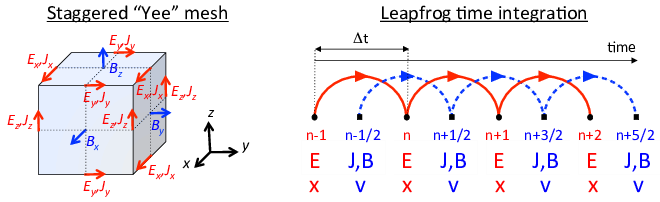
\includegraphics[scale=0.7]{figures/Yee_grid.png}
%\par\end{centering}
\caption{\label{fig:yee_grid}(left) Layout of field components on the staggered ``Yee'' grid. Current densities and electric fields are defined on the edges of the cells and magnetic fields on the faces. (right) Time integration using a second-order finite-difference "leapfrog" integrator.}
\end{figure}

The differential operator is defined as $\nabla=D_{x}\mathbf{\hat{x}}+D_{y}\mathbf{\hat{y}}+D_{z}\mathbf{\hat{z}}$
and the finite-difference operators in time and space are defined
respectively as $ $$D_{t}G|_{i,j,k}^{n}=\left(G|_{i,j,k}^{n+1/2}-G|_{i,j,k}^{n-1/2}\right)/\Delta t$$ $
and $D_{x}G|_{i,j,k}^{n}=\left(G|_{i+1/2,j,k}^{n}-G|_{i-1/2,j,k}^{n}\right)/\Delta x$,
where $\Delta t$ and $\Delta x$ are respectively the time step and
the grid cell size along $x$, $n$ is the time index and $i$, $j$
and $k$ are the spatial indices along $x$, $y$ and $z$ respectively.
The difference operators along $y$ and $z$ are obtained by circular
permutation. The equations in brackets are given for completeness,
as they are often not actually solved, thanks to the usage of a so-called
charge conserving algorithm, as explained below. As shown in Figure
\ref{fig:yee_grid}, the quantities are given on a staggered (or ``Yee'')
grid \cite{Yee}, where the electric field components are located
between nodes and the magnetic field components are located in the
center of the cell faces. Knowing the current densities at half-integer steps, 
the electric field components are updated alternately with the magnetic 
field components at integer and half-integer steps respectively.
